\problemname{Tour}
There are many tourist attractions in Toruń.
Our tour guides prepared a list of $m$ one-way walks connecting $n$ meeting points in the city center.
The walks are numbered from $1$ to $m$ and similarly the meeting points are numbered from 1 to $n$.
Each walk leads from one meeting point to another and allows the participants
to see a single attraction on the way. It might be possible to see the same attraction on different walks and
there might be mutliple walks between the same pair of meeting points.
We would like to organise an \emph{interesting tour} on our day off.

A \emph{tour} is a sequence of walks,
such that every walk starts at the meeting point where the previous one ends.
Furthermore, the last walk ends at the meeting point where the very first walk begins.

We call such a tour \emph{interesting} if
it doesn't contain the same attraction twice in a row.
In other words, every two consecutive walks from the tour allow us to see different attractions,
and additionally the very first and very last walks from the tour allow us to see different attractions as well.
Note that we do not mind if some non-consecutive walks allow us to see the same attraction.
In particular, the same walk might be used multiple times on the tour (but not twice in a row).

Your task is to check if it is possible to form an interesting tour, and if so to find one.
You can output any interesting tour that consists of at most $m$ walks.
It can be proven that if there exists an interesting tour, then there exists one consisting of at most $m$ walks.

\section*{Input}
The first line contains a positive integer $t$ ($1 \leq t \leq 5\cdot10^{5}$) denoting the number of test cases.

The first line of each test case contains positive integers $n$ and $m$ ($2\leq n$, $1\leq m$) denoting the number
of meeting points and walks, respectively.

Each of the subsequent $m$ lines describes one of the $m$ walks.
The $i$-th line contains three positive integers $x_{i}, y_{i}$ and $c_{i}$
($1\leq x_{i}, y_{i}\leq n$, $x_{i} \neq y_{i}$, $1\leq c_{i}\leq m$), which indicate that the $i$-th walk
starts at the meeting point $x_{i}$, ends at the meeting point $y_{i}$, and allows us to see the attraction $c_{i}$.

Let $N$ and $M$ denote the sum of $n$ and $m$, respectively, over all test cases. You can assume that $N, M \leq 10^{6}$.

\section*{Output}
For each test case, in the first line you should output \texttt{YES} if it is possible to organise an interesting tour
and \texttt{NO} otherwise. In the former case, the second line should first contain a positive integer $k$ ($2\leq k\leq m$) denoting
the number of walks forming the interesting tour. This should be followed by $k$ integers
$p_{1}, p_{2}, \ldots, p_{k}$
separated by single spaces. These numbers should describe an interesting tour, where we first follow walk
$p_{1}$, then $p_{2}$, and so on, and finally we follow walk $p_{k}$ returning to the original meeting point.

\section*{Scoring}
\begin{center}
\begin{tabular}{|l|l|l|}
\hline
\textbf{Subtask} & \textbf{Constraints} & \textbf{Points} \\\hline
1 & $m \leq 10$ and $t \leq 100$ & 9 \\\hline
2 & $M \leq 5000$ & 23 \\\hline
3 & $M \leq 5 \cdot 10^{4}$ & 19 \\\hline
4 & $M \leq 2 \cdot 10^{5}$ & 25 \\\hline
5 & No additional constraints. & 24 \\\hline
\end{tabular}
\end{center}

\section*{Explanation of sample 4}
\begin{figure}[h!]
    \centering
    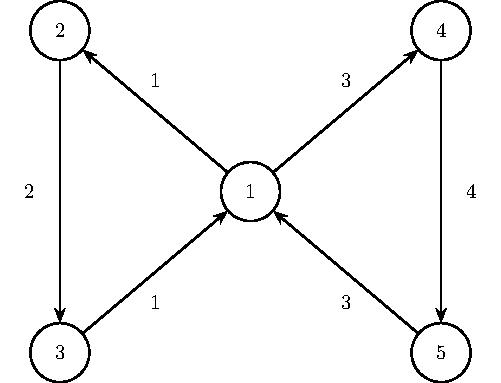
\includegraphics[width=0.6\textwidth]{sample.pdf}
    \caption{Illustration of sample 4. The arrows represent the walks between meeting points.}
\end{figure}
